\documentclass[tikz,border=10pt]{standalone}
\usepackage{tikz}
\usetikzlibrary{positioning, arrows.meta, shapes.geometric, backgrounds, fit}

\begin{document}
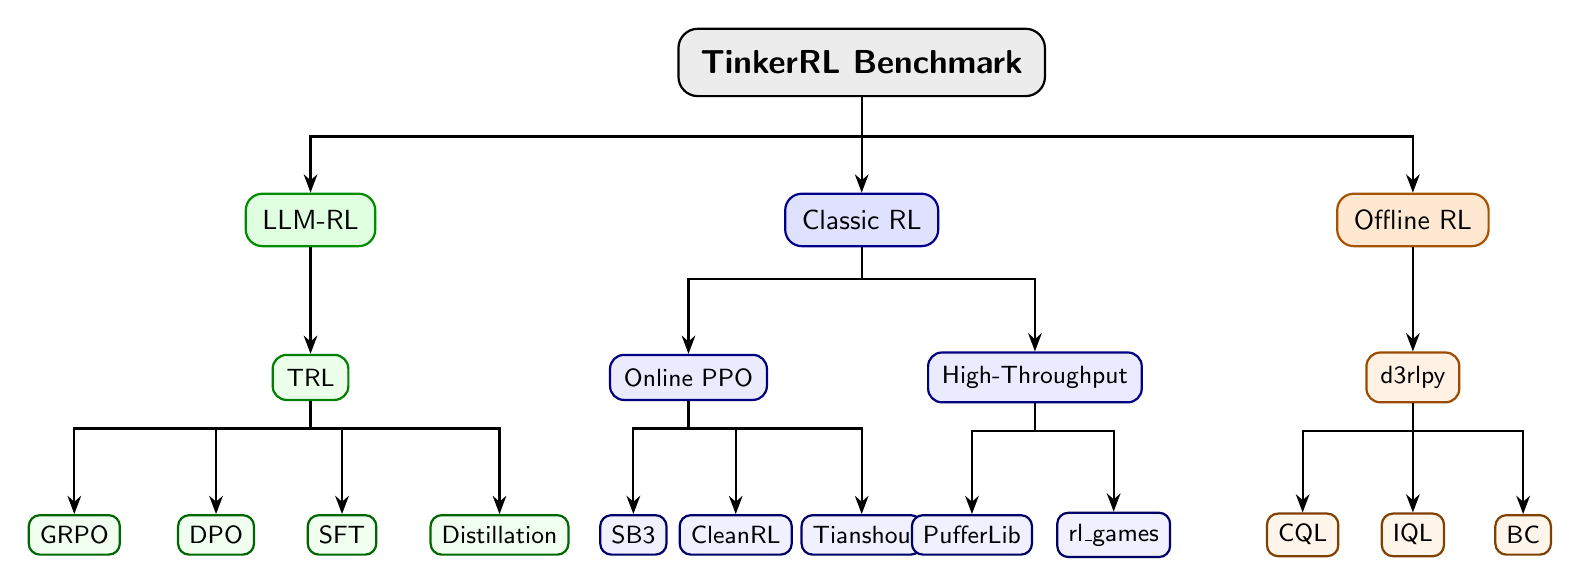
\begin{tikzpicture}[
  font=\sffamily,
  >=Stealth,
  thick,
  %% Node styles
  root/.style={
    draw, rounded corners=7pt, fill=gray!15, thick,
    text=black, font=\sffamily\bfseries\large,
    inner sep=8pt, align=center
  },
  branch/.style={
    draw, rounded corners=6pt, thick,
    inner sep=6pt, align=center, font=\sffamily\normalsize
  },
  subbranch/.style={
    draw, rounded corners=5pt, thick,
    inner sep=5pt, align=center, font=\sffamily\small
  },
  leaf/.style={
    draw, rounded corners=4pt,
    inner sep=4pt, align=center, font=\sffamily\small
  },
  %% Colors
  llm/.style={fill=green!12, draw=green!55!black},
  classic/.style={fill=blue!12, draw=blue!55!black},
  offline/.style={fill=orange!18, draw=orange!65!black},
  llm-sub/.style={fill=green!8, draw=green!50!black},
  classic-sub/.style={fill=blue!8, draw=blue!50!black},
  offline-sub/.style={fill=orange!10, draw=orange!60!black},
  llm-leaf/.style={fill=green!6, draw=green!40!black},
  classic-leaf/.style={fill=blue!6, draw=blue!40!black},
  offline-leaf/.style={fill=orange!8, draw=orange!50!black},
]

%% ── ROOT ──────────────────────────────────────────────────────────────────
\node[root] (root) at (0, 0) {TinkerRL Benchmark};

%% ── LEVEL 1 ───────────────────────────────────────────────────────────────
\node[branch, llm]     (llm)     at (-7.0, -2.0) {LLM-RL};
\node[branch, classic] (classic) at ( 0.0, -2.0) {Classic RL};
\node[branch, offline] (offline) at ( 7.0, -2.0) {Offline RL};

%% Root → L1 edges
\foreach \ch in {llm, classic, offline}
  \draw[->, thick] (root.south) -- ++(0,-0.5) -| (\ch.north);

%% ── LEVEL 2 ───────────────────────────────────────────────────────────────
\node[subbranch, llm-sub]     (trl)  at (-7.0, -4.0) {TRL};
\node[subbranch, classic-sub] (ppo)  at (-2.2, -4.0) {Online PPO};
\node[subbranch, classic-sub] (high) at ( 2.2, -4.0) {High-Throughput};
\node[subbranch, offline-sub] (d3r)  at ( 7.0, -4.0) {d3rlpy};

%% L1 → L2 edges
\draw[->, thick] (llm.south) -- (trl.north);
\draw[->, thick] (classic.south) -- ++(0,-0.4) -| (ppo.north);
\draw[->, thick] (classic.south) -- ++(0,-0.4) -| (high.north);
\draw[->, thick] (offline.south) -- (d3r.north);

%% ── LEVEL 3: TRL leaves ───────────────────────────────────────────────────
\node[leaf, llm-leaf] (grpo) at (-10.0, -6.0) {GRPO};
\node[leaf, llm-leaf] (dpo)  at ( -8.2, -6.0) {DPO};
\node[leaf, llm-leaf] (sft)  at ( -6.6, -6.0) {SFT};
\node[leaf, llm-leaf] (dist) at ( -4.6, -6.0) {Distillation};

\foreach \lf in {grpo, dpo, sft, dist}
  \draw[->, thick] (trl.south) -- ++(0,-0.35) -| (\lf.north);

%% ── LEVEL 3: Online PPO leaves ────────────────────────────────────────────
\node[leaf, classic-leaf] (sb3)      at (-2.9, -6.0) {SB3};
\node[leaf, classic-leaf] (cleanrl)  at (-1.6, -6.0) {CleanRL};
\node[leaf, classic-leaf] (tianshou) at ( 0.0, -6.0) {Tianshou};

\foreach \lf in {sb3, cleanrl, tianshou}
  \draw[->, thick] (ppo.south) -- ++(0,-0.35) -| (\lf.north);

%% ── LEVEL 3: High-Throughput leaves ──────────────────────────────────────
\node[leaf, classic-leaf] (puffer)  at (1.4, -6.0) {PufferLib};
\node[leaf, classic-leaf] (rlgames) at (3.2, -6.0) {rl\_games};

\foreach \lf in {puffer, rlgames}
  \draw[->, thick] (high.south) -- ++(0,-0.35) -| (\lf.north);

%% ── LEVEL 3: d3rlpy leaves ────────────────────────────────────────────────
\node[leaf, offline-leaf] (cql) at (5.6, -6.0) {CQL};
\node[leaf, offline-leaf] (iql) at (7.0, -6.0) {IQL};
\node[leaf, offline-leaf] (bc)  at (8.4, -6.0) {BC};

\foreach \lf in {cql, iql, bc}
  \draw[->, thick] (d3r.south) -- ++(0,-0.35) -| (\lf.north);

\end{tikzpicture}
\end{document}
